\documentclass[a3paper,12pt]{article}
\usepackage[latin1]{inputenc}
\usepackage[spanish]{babel}
\usepackage{multicol}
\usepackage{multirow}
\usepackage{eurosym}
\usepackage{graphicx}
\usepackage{fancybox}
\usepackage[dvipsnames]{color}

% sacado de /usr/share/doc/texmf/latex/geometry/geometry.dvi.gz
% para definir tipo de hoja y m�rgenes (90% texto, 5% margen izqdo, 5 drcho)
\usepackage[verbose,noheadfoot,dvips,a3paper,hscale=1,vscale=1]{geometry}

% cogidos de la presentacion
\newcommand{\LyX}{L\kern-.1667em\lower.25em\hbox{Y}\kern-.125emX\@}
\newcommand{\cila}{{\sc Curso de Introducci�n a Linux para Alumnos}}
%\newcommand{\pila}{{\sc Party de Instalaci�n de Linux para Alumnos}}
%\newcommand{\tila}{{\sc Taller de Iniciaci�n a Linux para Alumnos}}
\newcommand{\gulic}{{\sc Grupo de Usuarios de Linux de Canarias}}
\newcommand{\fmat}{{\sc Facultad de Matem�ticas}}
\newcommand{\ull}{{\sc Universidad de La Laguna}}
\newcommand{\linux}{GNU/Linux}
\newcommand{\debian}{Debian \linux}
\newcommand{\gfdl}{GNU Free Documentation License}
\newcommand{\myoval}[1]{\vspace*{3mm}\Ovalbox{\parbox{\columnwidth}{\large\sf #1}}\vspace*{3mm}}
\newcommand{\MYOVAL}[1]{\Ovalbox{\parbox{\columnwidth}{\LARGE\bf\sf #1}}\vspace*{2mm}}
\newcommand{\dcha}[1]{\vspace*{-7mm}\begin{flushright}#1\end{flushright}\vspace*{-4mm}}

\setlength{\parskip}{2mm}
\setlength{\columnsep}{10mm}
\setlength{\fboxsep}{2mm}
\setlength{\fboxrule}{1mm}

\begin{document}
\thispagestyle{empty}


%\vspace*{3mm}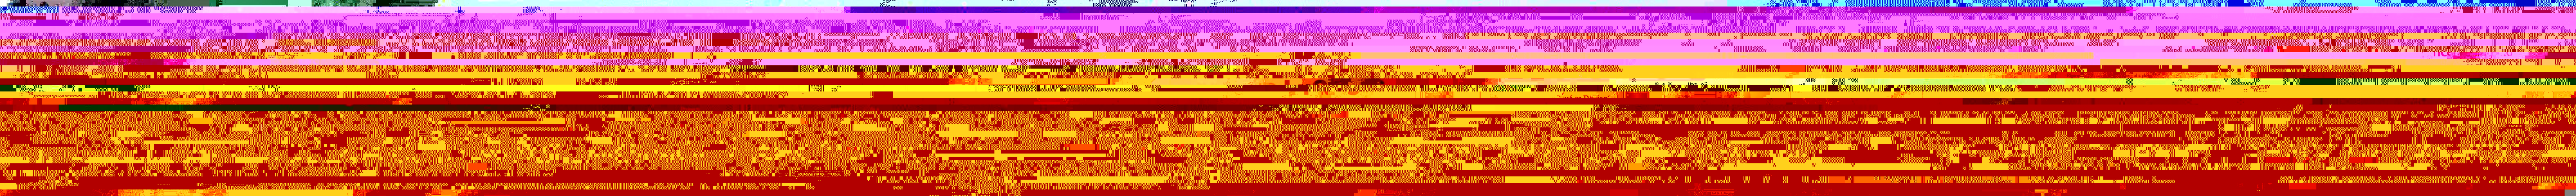
\includegraphics[width=285mm]{imagenes/barratotal.eps}

\vspace*{0.5cm}
%\rotatebox{90}{\resizebox{100mm}{10mm}{\Large\bf Del 18 al 22 de septiembre del2006}}

\vspace*{-8.7cm}
\hspace*{-6mm}\includegraphics{imagenes/cila_encuentro50_logos.eps}

\vspace*{-16.5cm}
\vspace*{-18.5cm}\hspace*{2.5cm}

\vspace*{-9cm} %Bug1:::: Comentario a�adido para corregir algo a lo chapuza.
\hspace*{17cm} 

\hspace*{25mm}
\begin{minipage}{25cm}

%
\includegraphics[width=100mm]{imagenes/fecha.eps}
\vspace*{1 cm}
\resizebox{100mm}{15mm}{\Large\bf \textcolor{white}{Del 28 de octubre al 2 de diciembre}}
\resizebox{75mm}{40mm}{\Large\bf \textcolor{white}{CILA}}

%
\includegraphics[width=100mm]{imagenes/cila.gulic.org.eps}

%\vspace*{35mm}
\vspace*{1 cm}

\myoval{�Qu� es?} 
  \large
	\par \noindent El CILA (Curso de Introducci�n a Linux para Alumnos) es un
curso que tradicionalmente a estado destinado a ``usuarios novatos''. Por ``usuarios
novatos'' entendemos gente que no use habitualmente o desconozca este sistema
operativo as� como el software libre en general. Este a�o, adem�s, ofrecemos otros cursos m�s espec�ficos. 

\myoval{Curso Iniciaci�n (2 cle).}
	\par \noindent Su finalidad es dotar a los alumnos que desconozcan el sistema operativo Linux o el software libre en general de los conocimientos m�nimos que les permitan desenvolverse con soltura en este entorno. Aprender�n herramientas de software
libre mediante charlas y de forma pr�ctica con las que puedan realizar sus trabajos acad�micos u otras actividades sobre esta plataforma.\\\\
\myoval{Curso Administraci�n Sistemas Linux (2 cle).}
  \par \noindent Curso orientado a aquellos usuarios que deseen aprender a dar distintos tipos de servicios con un sistema GNU/Linux. Se requiere que se tenga cierta soltura a la hora de manejar este sistema desde el punto de vista de usuario.

\myoval{Curso Programaci�n Phyton (1 cle).}
  \par  \noindent Curso orientado a hacer aplicaciones de escritorio, trabajar con bases de datos y plataformas web usando como lenguaje de programaci�n python. Para matricularse de este curso no es indespensable saber programar en python, pero si el programar con soltura en alg�n otro lenguaje, puesto que se avanzara muy r�pido en el curso.

\myoval{Curso Herramientas T�cnico Cient�ficas (1 cle).}
  \par \noindent Talleres en el que se introducir�n herramientas necesarias para los primeros a�os de la titulaci�n de matem�ticas, aunque las herramientas vistas pueden ser �tiles tambi�n en f�sica y en ingenier�as.

\myoval{Fechas, horario y lugar} 
Los cursos se realizar�n los s�bados comprendidos entre el 28 de octubre y el 2 de diciembre del 2006 en horario de 9:00 a 14:30. En el edificio blanco y en el edificio Calabaza de las Facultades de Matem�ticas y F�sica de la Universidad de La Laguna.
\begin{center}
	\Large \par \noindent \begin{tabular}{ccccc}
 	\textbf{Curso}     & \textbf{Plazas}   & \textbf{D�as(octubre)} & \textbf{D�as(noviembre)} & \textbf{D�as(diciembre)} \\
	 Iniciaci�n		     &  50               &  28                    & 4, 11, 18                &                          \\
   Administraci�n    &  20               &  28                    & 4, 11, 18                &                          \\
   P.Python          &  25               &                        & 25                       &  2                       \\
   H.T.Cient�ficas   &  25               &                        & 25                       &  2   										\\         
	\end{tabular} \\
\end{center}

\end{minipage}

%\vspace*{10mm}

\vspace*{6mm}\hspace*{2mm}\parbox{30cm}{%
\centering\Huge\sf
%Matr�cula abierta del 9 al 17 de Septiembre en la oficina del \\
%Vicerrectorado de Extensi�n Universitaria, en C/ Viana, 50}
M�s informaci�n sobre los contenidos de los cursos as� como la matr�cula 
\\en la URL \textcolor{blue}{\tt http://cila.ssl.ull.es} o escribiendo a \\ 
\textcolor{blue}{\tt cila@gulic.org}}


\end{document}
